\documentclass[a4paper,11pt]{article}

% --- Preamble ---
\usepackage[utf8]{inputenc}
\usepackage[T1]{fontenc}
\usepackage[indonesian]{babel}
\usepackage{geometry}
\geometry{margin=1in}
\usepackage{amsmath, amssymb, amsthm}
\usepackage{graphicx}
\usepackage{booktabs}
\usepackage{hyperref}
\usepackage{xcolor}
\usepackage{titlesec}
\usepackage{enumitem}
\usepackage{tikz}
\usetikzlibrary{shapes.geometric, arrows.meta, positioning, fit, backgrounds}

% Custom Colors
\definecolor{darkblue}{RGB}{0, 51, 102}
\hypersetup{
    colorlinks=true,
    linkcolor=darkblue,
    filecolor=magenta,      
    urlcolor=cyan,
    pdftitle={BTC-QUANT: Evolusi Model & Landasan Ekonofisika},
}

\title{
    \textbf{\huge BTC-QUANT SCALPING SYSTEM}\\
    \large Evolusi Arsitektur Strategi: Dari Markovian ke Bayesian Ekonofisika
}
\author{Saeful Ismail \& Miftah Farid Mahardika}
\date{\today}

\begin{document}

\maketitle

\begin{abstract}
Laporan teknis ini mendokumentasikan perjalanan pengembangan sistem trading \textit{high-frequency scalping} untuk instrumen Bitcoin. Fokus utama dokumen ini adalah transisi arsitektur dari model \textit{Hidden Markov Model} (HMM) yang bersifat kaku menuju sistem berbasis \textit{Bayesian Online Changepoint Detection} (BCD) yang didasarkan pada prinsip-prinsip ekonofisika. Kami menyajikan hasil validasi \textit{Golden Model} v4.4 yang menunjukkan stabilitas performa jangka panjang dengan \textit{Sharpe Ratio} > 2.0 dan \textit{Max Drawdown} terkendali.
\end{abstract}

\tableofcontents
\newpage

% --- Sections ---
\section{Pendahuluan}
\label{sec:intro}

Pasar \textit{futures} Bitcoin merupakan salah satu instrumen keuangan dengan karakteristik paling menantang untuk dimodelkan secara algoritmik. Volatilitas hariannya yang dapat mencapai 10--20\% dalam satu sesi, distribusi \textit{return} yang bercirikan \textit{fat-tail} (jauh dari asumsi Gaussian), serta sifat \textit{non-stationary} yang menyebabkan perubahan regime pasar secara mendadak --- semuanya menjadikan pendekatan \textit{machine learning} konvensional sering kali tidak memadai.

Penelitian ini mempresentasikan \textbf{BTC-QUANT}, sebuah sistem \textit{scalping} algoritmik yang dibangun di atas fondasi \textbf{ekonofisika} --- cabang ilmu yang meminjam kerangka berpikir fisika statistik untuk memodelkan dinamika pasar finansial. Kontribusi utama ekonofisika dalam sistem ini terletak pada \textbf{Layer 1: \textit{Bayesian Changepoint Detection} (BCD)}, yang memperlakukan perubahan regime pasar sebagai \textit{phase transition} --- analog dengan perubahan fase dalam sistem fisik --- alih-alih sebagai transisi probabilistik statis seperti pada model Markovian.

\subsection{Motivasi dan Rumusan Masalah}

Pertanyaan penelitian yang mendasari pengembangan BTC-QUANT adalah:
\begin{enumerate}
    \item Dapatkah pendekatan berbasis \textit{structural break} (BCD) mengungguli model \textit{clustering} global (HMM) dalam mendeteksi regime pasar kripto secara prediktif?
    \item Apakah arsitektur multi-lapis yang memisahkan deteksi regime, konfirmasi teknikal, kecerdasan buatan, dan filter volatilitas dapat menghasilkan profil risiko-pengembalian yang superior dibandingkan pendekatan \textit{single-model}?
    \item Pada titik kompleksitas mana penambahan fitur justru memperburuk performa (\textit{alpha decay})?
\end{enumerate}

\subsection{Latar Belakang: Era Hidden Markov Model}
Pada tahap awal riset, kami mencoba menerapkan \textit{Gaussian Hidden Markov Model} (HMM) untuk mendeteksi rezim pasar sesuai dengan metodologi standar dalam pengolahan sinyal \cite{rabiner1989tutorial}. Hipotesis awalnya adalah harga bersifat Markovian, di mana status pasar (bullish, bearish, sideways) dapat diestimasi dari observasi \textit{return} dan volume.

\begin{figure}[h!]
    \centering
    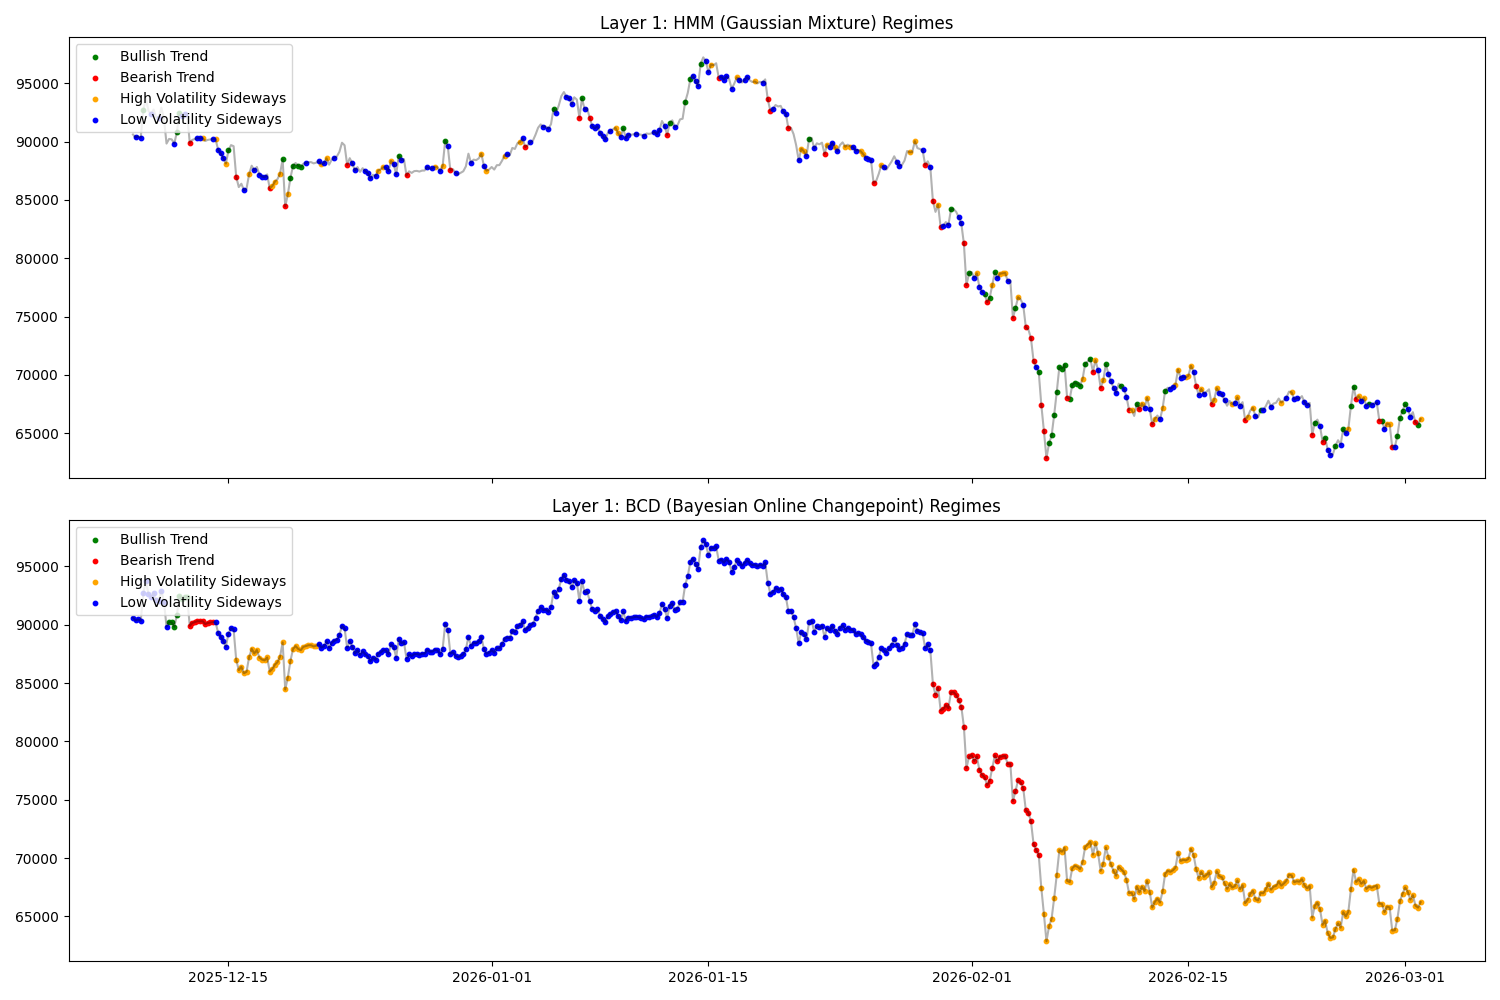
\includegraphics[width=0.8\textwidth]{figures/bcd_vs_hmm.png}
    \caption{Perbandingan Visual antara Deteksi Rezim HMM (Legacy) dan BCD (Ekonofisika).}
    \label{fig:hmm_vs_bcd}
\end{figure}

\subsection{Kegagalan Model Markovian}
Setelah melalui berbagai iterasi (\textit{Standard HMM}, \textit{Non-Homogeneous HMM}, dan \textit{GMM-HMM}), kami menemukan beberapa kelemahan fundamental:
\begin{enumerate}
    \item \textbf{Transition Rigidity:} Probabilitas transisi yang statis gagal menangkap perubahan mendadak akibat faktor eksternal seperti \textit{liquidation cascades} atau perubahan \textit{funding rate}.
    \item \textbf{High Latency/Bottleneck:} Model yang lebih kompleks (NHHM) membutuhkan waktu kalibrasi yang tidak realistis untuk sistem \textit{scalping} (berjam-jam per siklus).
    \item \textbf{Predictive Failure:} Melalui pengujian \textit{Walk-Forward} (Modul C), HMM secara konsisten gagal melewati ambang batas signifikansi statistik \textit{out-of-sample}.
\end{enumerate}

Kegagalan ini memicu pergeseran paradigma dari \textit{Machine Learning} murni ke arah pendekatan yang lebih fundamental: \textbf{Ekonofisika}.

\subsection{Struktur Dokumen}

Dokumen ini disusun sebagai berikut: Bab~\ref{sec:theory} menjelaskan landasan teoritis ekonofisika dan formulasi matematis BCD. Bab~\ref{sec:architecture} mendeskripsikan arsitektur 6-\textit{layer pipeline} secara menyeluruh. Bab~\ref{sec:evolution} mendokumentasikan evolusi sistem dari v0.1 hingga v4.5 beserta justifikasi empiris setiap transisi. Bab~\ref{sec:results} menyajikan validasi statistik komprehensif termasuk pengujian lintas regime dan perbandingan longitudinal. Bab~\ref{sec:conclusion} merangkum temuan dan memaparkan \textit{roadmap} pengembangan selanjutnya.

\section{Landasan Ekonofisika: Bayesian Changepoint Detection}
\label{sec:theory}

Ekonofisika memandang pasar finansial bukan sebagai sistem acak murni, melainkan sebagai sistem kompleks non-ekuilibrium yang mengalami transisi fase. Arsitektur BTC-QUANT mengadopsi pandangan ini dengan mengganti model \textit{clustering} global (HMM) menjadi deteksi patahan struktur lokal secara \textit{online}.

\subsection{Filosofi Patahan Struktur (Phase Transitions)}
Dalam fisika, sistem berpindah fase (seperti air menjadi es) saat mencapai titik kritis \cite{mantegna1999introduction}. Di pasar kripto, perubahan tren dari \textit{bullish} ke \textit{bearish} atau sebaliknya sering kali terjadi secara mendadak melalui lonjakan volatilitas. Algoritma \textit{Bayesian Online Changepoint Detection} (BCD) \cite{adams2007bayesian} dirancang untuk mendeteksi "retakan" ini secara \textit{real-time}.

\subsection{Formulasi Bayesian Online Changepoint Detection}
BCD bekerja dengan menghitung distribusi probabilitas dari \textit{Run Length} ($r_t$), yaitu durasi sejak terjadinya titik patahan (\textit{changepoint}) terakhir. Probabilitas posisi saat ini berada pada \textit{run length} tertentu dinyatakan sebagai:

\begin{equation}
    P(r_t | y_{1:t}) = \frac{\sum_{r_{t-1}} P(r_t | r_{t-1}) P(y_t | r_{t-1}, y_{t}^{(r)}) P(r_{t-1} | y_{1:t-1})}{\sum_{r_t} P(r_t | y_{1:t})}
\end{equation}

Di mana:
\begin{itemize}
    \item $P(r_t | r_{t-1})$ adalah \textit{Hazard Function} yang menentukan probabilitas terjadinya \textit{reset} (changepoint).
    \item $P(y_t | r_{t-1}, y_{t}^{(r)})$ adalah \textit{Predictive Posterior}, yaitu probabilitas data baru ($y_t$) berdasarkan riwayat data dalam rezim saat ini.
\end{itemize}

Jika data baru sangat tidak konsisten dengan distribusi saat ini, probabilitas \textit{run length} kembali ke nol ($r_t = 0$) akan melonjak, menandakan dimulainya rezim baru.

\subsection{Mengatasi Fat-Tails dengan Distribusi Student-T}
Salah satu kontribusi ekonofisika yang paling krusial adalah pengakuan atas distribusi non-Gaussian (\textit{Lévy Flights}) \cite{mandelbrot2010misbehavior}. Pasar kripto sering kali mengalami pergerakan ekstrem yang tidak mungkin dijelaskan oleh kurva lonceng normal standar.

Dalam implementasi BTC-QUANT, kami mengganti fungsi distribusi normal pada \textit{Predictive Posterior} BCD dengan \textbf{Student-T Predictive Posterior}:

\begin{equation}
    y_t | \mathcal{D}_{t-1} \sim St(\mu_{t-1}, \lambda_{t-1}, \nu_{t-1})
\end{equation}

Distribusi Student-T memiliki parameter \textit{degrees of freedom} ($\nu$) yang memungkinkan model memiliki \textit{kurtosis} lebih tinggi. Secara teknis, ini memungkinkan bot untuk menyerap "noise" atau anomali harga jangka pendek tanpa langsung menghancurkan model rezim yang sedang berjalan.

\subsection{Local Parameter Estimation}
Berbeda dengan HMM yang mencoba mencari satu set parameter global untuk seluruh data historis (stasioner), BCD melakukan estimasi parameter secara lokal. Model hanya peduli pada data \textit{sejak titik changepoint terakhir}. Hal ini membuat sistem kita mengakui bahwa "sifat fisika" pasar hari ini bisa sangat berbeda dengan bulan lalu, sebuah konsep yang dikenal sebagai \textit{Non-Equilibrium Dynamics}.

\section{Arsitektur Sistem: 6-Layer Pipeline}
\label{sec:architecture}

Sistem BTC-QUANT dibangun di atas arsitektur modular enam lapis (\textit{6-Layer Pipeline}) yang mentransformasi data pasar mentah menjadi sinyal eksekusi yang tervalidasi secara statistik.

 \subsection{Ikhtisar Signal Stack}
Setiap lapisan dalam sistem ini memiliki tanggung jawab spesifik yang saling mengonfirmasi:
\begin{itemize}
    \item \textbf{Layer 1 (Regime Detection):} Menggunakan BCD (seperti yang dijelaskan pada Bab 2) untuk menentukan bias arah pasar.
    \item \textbf{Layer 2 (Technical Alignment):} Memastikan konfluensi antara harga saat ini dengan \textit{Exponential Moving Average} (EMA 20 dan 50).
    \item \textbf{Layer 3 (AI Intelligence):} Menggunakan \textit{Multi-Layer Perceptron} (MLP) yang dilatih secara \textit{online} untuk memprediksi probabilitas arah lilin berikutnya.
    \item \textbf{Layer 4 (Volatility Gate):} Filter berbasis rasio volatilitas ATR yang memblokir entri pada kondisi pasar \textit{high-chaos}. Model Heston stokastik diintegrasikan penuh pada v4.5 (R\&D).
\end{itemize}

\begin{figure}[h!]
\centering
\begin{tikzpicture}[
    every node/.style = {align=center},
    box/.style = {
        rectangle, rounded corners=4pt,
        minimum width=8cm, minimum height=0.9cm,
        text centered, font=\small
    },
    layer/.style    = {box, draw=darkblue, fill=blue!8, text=darkblue},
    decision/.style = {box, draw=orange!70!black, fill=orange!12, text=orange!80!black},
    outbox/.style   = {rectangle, rounded corners=4pt,
                       minimum width=3.6cm, minimum height=0.9cm,
                       text centered, font=\small},
    input/.style    = {box, draw=gray!60, fill=gray!10, text=black},
    arrow/.style    = {-{Stealth[length=5pt]}, thick, darkblue},
    skiparrow/.style= {-{Stealth[length=5pt]}, thick, red!60!black, dashed},
]

% --- Pipeline utama (vertikal, x=0) ---
\node[input]    (data) at (0, 0)
    {Data Pasar: BTC/USDT 4H OHLCV};
\node[layer]    (l1)   at (0,-1.6)
    {\textbf{Layer 1 --- Regime Detection}\\
     \footnotesize BCD + Student-T Posterior};
\node[layer]    (l2)   at (0,-3.2)
    {\textbf{Layer 2 --- Technical Alignment}\\
     \footnotesize EMA 20/50 Confluence Check};
\node[layer]    (l3)   at (0,-4.8)
    {\textbf{Layer 3 --- AI Intelligence}\\
     \footnotesize MLP Online-Trained: Probabilitas Arah Candle};
\node[layer]    (l4)   at (0,-6.4)
    {\textbf{Layer 4 --- Volatility Gate}\\
     \footnotesize $\mathrm{ATR}_{14}/\mathrm{price}_t \;\rightarrow\;$ Vol Multiplier};
\node[decision] (spec) at (0,-8.0)
    {\textbf{Directional Spectrum Score}\\
     \footnotesize Weighted Voter Alignment (L1--L4)};
\node[decision] (gate) at (0,-9.6)
    {\textbf{Trade Gate}\\
     \footnotesize ACTIVE \;/\; ADVISORY \;/\; INACTIVE};

% --- Output nodes (vertikal di bawah gate, digeser kiri/kanan) ---
\node[outbox, draw=red!60!black, fill=red!8, text=red!70!black]
    (skip) at (-3.2,-12.4)
    {\textbf{SKIP}\\
     \footnotesize Tidak Ada Entri};
\node[outbox, draw=green!50!black, fill=green!10, text=green!40!black]
    (exec) at ( 3.2,-12.4)
    {\textbf{EXECUTE}: LONG / SHORT\\
     \footnotesize SL 1.333\% \; TP 0.71\% \; 6c};

% --- Panah pipeline utama ---
\draw[arrow] (data) -- (l1);
\draw[arrow] (l1)   -- (l2);
\draw[arrow] (l2)   -- (l3);
\draw[arrow] (l3)   -- (l4);
\draw[arrow] (l4)   -- (spec);
\draw[arrow] (spec) -- (gate);

% --- Percabangan dari gate ---
% turun dari gate ke titik cabang
\draw[darkblue, thick] (gate.south) -- (0,-11.5);
% cabang kiri ke SKIP
\draw[skiparrow] (0,-11.5) -| (skip.north)
    node[pos=0.25, above, font=\footnotesize, text=red!60!black] {INACTIVE};
% cabang kanan ke EXECUTE
\draw[arrow] (0,-11.5) -| (exec.north)
    node[pos=0.25, above, font=\footnotesize, text=green!40!black] {ACTIVE/ADVISORY};

\end{tikzpicture}
\caption{Arsitektur \textit{Signal Pipeline} BTC-QUANT v4.4. Data pasar diproses secara berurutan melalui empat layer sebelum mencapai \textit{Trade Gate}. Entri hanya dieksekusi saat skor \textit{Directional Spectrum} memenuhi ambang batas ACTIVE atau ADVISORY.}
\label{fig:architecture}
\end{figure}

\subsection{Layer 4: \textit{Volatility Gate}}

Layer 4 berfungsi sebagai \textbf{\textit{Go/Stop Gate}} yang memfilter kondisi pasar bervolatilitas ekstrem sebelum sinyal dari L1--L3 dieksekusi. Implementasinya pada \textbf{v4.4 Golden Model} menggunakan rasio volatilitas berbasis ATR (\textit{Average True Range}) terhadap harga saat ini sebagai proksi kondisi pasar:

\begin{equation}
    \text{vol\_ratio} = \frac{\text{ATR}_{14}}{\text{price}_t}
\end{equation}

Nilai \textit{vol\_ratio} ini kemudian dikonversi menjadi \textit{multiplier} yang memodulasi skor \textit{Directional Spectrum}. Jika kondisi volatilitas terlalu ekstrem, skor akhir akan jatuh ke bawah ambang batas \textit{Trade Gate}, sehingga seluruh entri diblokir (\textit{SKIP}). Pendekatan ini sengaja dibuat sederhana dan deterministik untuk memastikan stabilitas sistem produksi.

\textbf{Catatan mengenai Model Heston:} Persamaan difusi volatilitas stokastik \textit{mean-reverting} Heston \cite{heston1993closed} ---

\begin{equation}
    dv(t) = -\gamma(v - \eta)\,dt + \kappa \sqrt{v}\, dB_v(t)
\end{equation}

--- diintegrasikan secara penuh pada \textbf{v4.5 Heston Adaptive} (fase R\&D), di mana SL/TP dikalkulasi secara adaptif berdasarkan estimasi volatilitas stokastik aktual. Pada v4.4, Layer 4 mengadopsi \textit{prinsip} mean-reversion volatilitas sebagai landasan konseptual, namun implementasinya menggunakan ATR sebagai aproksimasi yang lebih stabil untuk konteks produksi.

\subsection{Directional Spectrum \& Trade Gate}
Keputusan akhir diambil melalui integrasi suara (\textit{voter alignment}) dari ketiga lapisan pertama yang dimodulasi oleh pengali volatilitas dari Layer 4. Hasilnya adalah skor \textit{Directional Spectrum} yang diklasifikasikan ke dalam tiga gerbang (\textit{Trade Gate}):

\begin{enumerate}
    \item \textbf{ACTIVE:} Sinyal sangat kuat dan semua lapisan selaras (Win Rate tertinggi).
    \item \textbf{ADVISORY:} Sinyal moderat dengan konfirmasi cukup dari mayoritas lapisan.
    \item \textbf{INACTIVE:} Terjadi konflik sinyal antar lapisan atau filter volatilitas aktif (entri dilarang).
\end{enumerate}

Arsitektur ini memastikan bahwa bot hanya masuk ke dalam pasar saat terjadi konfluensi antara struktur harga fisik (L1), tren teknikal (L2), dan probabilitas kecerdasan buatan (L3) di bawah kondisi volatilitas yang stabil (L4).

\section{Evolusi Strategi: Dari v0.1 Menuju Golden Model v4.4}
\label{sec:evolution}

Pengembangan BTC-QUANT bukanlah sebuah proses linear, melainkan serangkaian iterasi \textit{trial-and-error} yang sistematis. Bab ini mendokumentasikan pelajaran empiris yang dipetik dari setiap fase pengujian --- mulai dari validasi fondasi algoritma hingga penemuan parameter perdagangan yang optimal. Seluruh pengujian pada fase evolusi ini dijalankan pada periode yang seragam (Januari 2024 -- Maret 2026) untuk memastikan perbandingan yang \textit{apples-to-apples} dan bebas dari bias pemilihan periode (\textit{period selection bias}).

% =========================================================
\subsection{v0.1 PoC: Validasi Awal Layer 1 BCD}

Titik awal pengembangan adalah \textit{Proof of Concept} (PoC) yang menggunakan hanya \textbf{Layer 1 BCD} sebagai satu-satunya filter sinyal, tanpa konfirmasi dari layer tambahan (L2--L4). Tujuannya adalah memvalidasi secara terisolasi apakah algoritma \textit{Bayesian Changepoint Detection} memiliki \textit{predictive power} yang memadai sebagai fondasi sistem sebelum kompleksitas ditambahkan.

Hasil pengujian menunjukkan bahwa fondasi BCD terbukti valid: \textit{Win Rate} mencapai 58.98\%, \textit{Net PnL} +312\%, dan \textit{Max Drawdown} terjaga pada 23.1\%. Namun terdapat satu kelemahan struktural yang jelas --- sistem melewatkan 1.855 candle (\textit{skip rate} tinggi) karena absennya mekanisme konfirmasi \textit{entry}. Peluang yang terlewatkan ini sangat terkonsentrasi pada kondisi \textit{bear market}, di mana \textit{Win Rate} hanya mencapai 56.1\%.

\textbf{Kesimpulan v0.1:} BCD terbukti sebagai fondasi sinyal yang kuat dan layak secara statistik, namun memerlukan layer konfirmasi tambahan untuk mengoptimalkan seleksi \textit{entry} dan mengurangi \textit{skip rate}.

% =========================================================
\subsection{Krisis v1: Jebakan \textit{Compounding} dan Risiko Ekor}

Merespons kelemahan v0.1, seluruh \textit{stack} L1--L4 diaktifkan pada v1 dengan tetap mempertahankan mekanisme \textit{compounding position sizing}. Hasilnya, jumlah \textit{trade} meningkat dari 958 menjadi 1.257 (\textit{skip rate} turun ke 1.113 candle) dan \textit{Net PnL} melonjak menjadi +676\%. Secara nominal, ini tampak sebagai kemajuan yang signifikan.

Namun di balik angka tersebut tersimpan profil risiko yang jauh lebih berbahaya:
\begin{itemize}
    \item \textbf{MDD Melonjak 56\%:} \textit{Max Drawdown} meningkat dari 23.1\% menjadi 35.95\% --- melampaui ambang batas operasional yang dapat diterima.
    \item \textbf{Risk Spiral:} Mekanisme \textit{compounding} memperbesar ukuran posisi seiring akumulasi profit, sehingga saat \textit{losing streak} terjadi, kerugian nominal per \textit{trade} ikut membesar secara proporsional, menciptakan spiral degradasi modal yang akseleratif.
    \item \textbf{Bear Regime Memburuk:} \textit{Win Rate} pada kondisi \textit{bear market} justru turun dari 56.1\% menjadi 53.9\% meskipun layer konfirmasi tambahan diaktifkan, mengindikasikan bahwa L2--L4 tidak memberikan nilai tambah yang signifikan pada regime ini.
\end{itemize}

\begin{table}[h!]
\centering
\caption{Perbandingan v0.1 vs v1: \textit{Trade-off} \textit{Return} vs Risiko (Periode 2024--2026)}
\label{table:v0_vs_v1}
\begin{tabular}{@{}lllllll@{}}
\toprule
\textbf{Versi} & \textbf{Net PnL} & \textbf{WR} & \textbf{PF} & \textbf{MDD} & \textbf{Sharpe} & \textbf{Sizing} \\ \midrule
v0.1 (L1 Only)  & +312\%  & 58.98\% & 1.139 & 23.10\%  & 1.396 & \textit{Compound} \\
v1 (Full Stack) & +676\%  & 58.07\% & 1.154 & 35.95\%  & 1.437 & \textit{Compound} \\
\bottomrule
\end{tabular}
\end{table}

Tabel~\ref{table:v0_vs_v1} memperlihatkan bahwa aktivasi penuh L2--L4 hanya meningkatkan \textit{Profit Factor} sebesar 0.015 dan \textit{Sharpe Ratio} sebesar 0.041, sementara MDD meningkat lebih dari 12 poin persentase. Ini adalah \textit{trade-off} yang secara kuantitatif tidak proporsional.

\textbf{Pelajaran v1:} Di pasar aset kripto yang bercirikan volatilitas tinggi dan distribusi \textit{fat-tail}, perlindungan modal melalui pengendalian \textit{drawdown} jauh lebih bernilai daripada potensi keuntungan nominal yang eksponensial namun tidak stabil.

% =========================================================
\subsection{v3 Baseline: Penyelamatan Melalui \textit{Fixed Position Sizing}}

Revisi fundamental dilakukan pada versi 3 dengan mengganti mekanisme \textit{compounding} menjadi \textbf{\textit{Fixed Position Sizing}} (margin tetap \$1.000 per \textit{trade}). Hasilnya sangat signifikan: MDD terpangkas hampir separuhnya menjadi 22.5\% --- hanya dengan mengubah aturan manajemen risiko tanpa menyentuh logika sinyal sama sekali. Temuan ini menegaskan bahwa \textit{position sizing} adalah variabel risiko yang lebih dominan dibandingkan kompleksitas sinyal itu sendiri.

% =========================================================
\subsection{Pelajaran \textit{Alpha Decay}: v4.2 dan v4.3}

Dengan fondasi \textit{fixed sizing} yang lebih aman, upaya berikutnya adalah meningkatkan kualitas sinyal melalui penambahan filter teknikal yang ketat, seperti konfirmasi \textit{Daily EMA 200} dan ambang batas \textit{Z-Score}. Alih-alih menghasilkan perbaikan, eksperimen ini justru mengungkap fenomena yang dikenal sebagai \textbf{\textit{Alpha Decay}}:
\begin{itemize}
    \item Filter yang terlalu restriktif memblokir sebagian besar sinyal masuk, termasuk sinyal yang secara historis menguntungkan.
    \item Frekuensi \textit{trade} yang menurun drastis mengakibatkan penurunan total \textit{return} meskipun \textit{win rate} per \textit{trade} secara individual tetap tinggi.
\end{itemize}

Temuan ini membuktikan bahwa pada sistem perdagangan berbasis momentum seperti BTC-QUANT, \textit{alpha} sejati berasal dari kualitas sinyal berlapis (L1--L4), bukan dari penambahan filter tambahan yang bersifat \textit{post-hoc}. Semakin banyak filter yang ditumpuk, semakin banyak \textit{alpha} yang terkikis.

% =========================================================
\subsection{v4.4 Golden Model: Konvergensi Menuju \textit{Baseline} Murni}

Puncak dari evolusi ini adalah \textbf{v4.4 Golden Model}. Berdasarkan evidens empiris dari fase-fase sebelumnya, diambil keputusan untuk mengeliminasi seluruh fitur manajemen posisi eksperimental seperti \textit{Breakeven Lock} dan \textit{Early Loss Exit}, dan kembali ke eksekusi yang murni berbasis sinyal.

Filosofi desain v4.4 bertumpu pada dua prinsip:
\begin{enumerate}
    \item \textbf{Kepercayaan pada Akurasi Sinyal:} Sistem mengandalkan akurasi \textit{entry} dari \textit{signal stack} L1--L4 yang secara empiris telah terbukti menghasilkan \textit{Win Rate} $>$58\%.
    \item \textbf{\textit{Natural Resolution}:} Setiap \textit{trade} dibiarkan berakhir secara alami melalui target \textit{Stop Loss} (1.333\%) atau \textit{Take Profit} (0.71\%), dengan batas waktu keamanan (\textit{safety timeout}) 24 jam (6 candle) untuk mencegah eksposur berlebih.
\end{enumerate}

Filosofi minimalis ini terbukti memberikan profil stabilitas tertinggi dalam seluruh sejarah pengujian, menghasilkan sistem yang tidak hanya menguntungkan secara konsisten tetapi juga memiliki perilaku yang dapat diprediksi (\textit{predictable stability}).

% =========================================================
\subsection{v4.5 Heston Adaptive: Eksperimen Volatilitas Dinamis}
\label{subsec:v45_heston}

Setelah v4.4 menetapkan \textit{baseline} yang stabil, dilakukan eksperimen lanjutan untuk menguji hipotesis berikut: \textit{apakah penggantian parameter SL/TP statis dengan nilai adaptif berbasis model volatilitas dapat meningkatkan kualitas eksekusi tanpa mengorbankan stabilitas?} Lahirlah \textbf{v4.5 Heston Adaptive} --- varian eksperimental yang mengintegrasikan model volatilitas stokastik \textit{mean-reverting} Heston untuk kalibrasi SL/TP secara dinamis, serta menerapkan \textit{dynamic position sizing} berbasis Kriteria Kelly (2\% ekuitas per \textit{trade}).

Perbedaan arsitektur antara kedua model dirangkum sebagai berikut:
\begin{itemize}
    \item \textbf{Golden v4.4:} SL tetap 1.333\%, TP tetap 0.71\%, \textit{leverage} 15$\times$, margin \$1.000/\textit{trade}.
    \item \textbf{Heston v4.5:} SL/TP adaptif berbasis ATR $\times$ \textit{multiplier} Heston, \textit{dynamic sizing} 2\% ekuitas/\textit{trade}, \textit{leverage} maksimum 5$\times$.
\end{itemize}

\subsubsection{Pengujian Jangka Pendek: 62 Hari (Januari--Maret 2026)}

Pengujian pertama dilakukan pada jendela waktu pendek (62 hari) untuk mengisolasi kualitas sinyal tanpa distorsi efek \textit{compounding} jangka panjang.

\begin{table}[h!]
\centering
\caption{Perbandingan Performa: Golden v4.4 vs Heston v4.5 (62 Hari, Jan--Mar 2026)}
\label{table:evo_62d}
\begin{tabular}{@{}llll@{}}
\toprule
\textbf{Metrik}         & \textbf{Golden v4.4} & \textbf{Heston v4.5}  & \textbf{Unggul} \\ \midrule
Net PnL (\%)            & +30.04\%             & \textbf{+76.10\%}     & Heston \\
\textit{Final Equity} (USD) & \$13.004         & \textbf{\$17.610}     & Heston \\
\textit{Win Rate}       & \textbf{57.36\%}     & 49.35\%               & Golden \\
\textit{Profit Factor}  & 1.278                & \textbf{1.587}        & Heston \\
\textit{Max Drawdown}   & 20.75\%              & \textbf{17.10\%}      & Heston \\
\textit{Sharpe Ratio}   & 2.299                & \textbf{3.409}        & Heston \\
R:R \textit{Ratio}      & 0.950                & \textbf{1.629}        & Heston \\
Jumlah \textit{Trade}   & \textbf{129}         & 77                    & Golden \\
\textit{TIME\_EXIT Rate}& \textbf{7.0\%}       & 36.4\%                & Golden \\
\bottomrule
\end{tabular}
\end{table}

\textbf{Heston unggul pada 7 dari 9 metrik.} Keunggulan utama bersumber dari R:R yang secara struktural lebih baik (1.629 vs 0.950) dan mekanisme \textit{dynamic sizing} yang membatasi kerugian maksimal per \textit{trade} terhadap ekuitas berjalan. Namun terdapat satu peringatan kritis yang perlu dicermati: \textbf{36.4\% \textit{trade} Heston berakhir melalui TIME\_EXIT} (dibandingkan hanya 7.0\% pada Golden). Ini mengindikasikan bahwa target TP Heston terlalu ambisius untuk kondisi \textit{Low Volatility} yang mendominasi periode Januari--Maret 2026 --- seluruh 77 \textit{trade} Heston pada periode ini masuk dalam kategori \textit{regime} \textit{Low Vol}.

\subsubsection{Validasi Longitudinal: 7 Tahun (2019--2026)}

Untuk menguji ketahanan kedua model lintas siklus penuh Bitcoin --- mencakup \textit{bear market} 2019, \textit{bull run} 2020--2021, fase koreksi 2022, dan pemulihan 2023--2026 --- dilakukan pengujian pada 7 tahun data historis (2.619 hari, 13.783 candle 4H).

\begin{table}[h!]
\centering
\caption{Perbandingan Longitudinal: Golden v4.4 vs Heston v4.5 (2019--2026)}
\label{table:evo_7y}
\begin{tabular}{@{}llll@{}}
\toprule
\textbf{Metrik}              & \textbf{Golden v4.4} & \textbf{Heston v4.5}   & \textbf{Unggul} \\ \midrule
\textit{Final Equity} (USD)  & \$128.321            & \textbf{\$16.928.244}  & Heston \\
Net PnL (\%)                 & +1.183\%             & \textbf{+169.182\%}    & Heston \\
\textit{Win Rate}            & \textbf{58.43\%}     & 46.67\%                & Golden \\
\textit{Profit Factor}       & \textbf{1.372}       & 1.302                  & Golden \\
\textit{Max Drawdown}        & \textbf{12.40\%}     & 71.94\%                & Golden \\
\textit{Sharpe Ratio}        & \textbf{3.087}       & 1.007                  & Golden \\
R:R \textit{Ratio}           & 0.976                & \textbf{1.488}         & Heston \\
Jumlah \textit{Trade}        & 3.866                & 2.100                  & -- \\
\textit{TIME\_EXIT Rate}     & \textbf{5.4\%}       & 39.5\%                 & Golden \\
\bottomrule
\end{tabular}
\end{table}

Hasil ini menghadirkan paradoks yang menarik secara akademis: Heston menghasilkan ekuitas akhir \textbf{131$\times$ lebih besar} (\$16,9 juta vs \$128 ribu), namun kalah pada 6 dari 9 metrik kualitas. Penjelasannya terletak pada efek \textit{compounding} agresif selama 7 tahun --- setiap kemenangan Heston memperbesar basis modal untuk \textit{trade} berikutnya, menghasilkan pertumbuhan eksponensial yang secara inheren juga memperbesar eksposur risiko secara proporsional.

Keunggulan nominal tersebut datang dengan tiga konsekuensi yang tidak dapat diabaikan dalam konteks manajemen risiko:
\begin{itemize}
    \item \textbf{\textit{Max Drawdown} 71.94\%:} Pada titik terburuk, ekuitas dapat menyusut hingga 72\% dari nilai puncaknya. Kondisi ini secara psikologis dan operasional hampir mustahil dipertahankan tanpa intervensi, dan jauh melampaui toleransi risiko institusional manapun.
    \item \textbf{\textit{Sharpe Ratio} 1.007:} Berada di ambang batas minimum yang dianggap layak ($>$1.0). Volatilitas ekstrem mengikis nilai \textit{risk-adjusted return} hingga mendekati batas kelayakan.
    \item \textbf{\textit{High Vol Regime} Tidak Teruji:} Seluruh 2.100 \textit{trade} Heston dalam periode 7 tahun dikategorikan sebagai regime \textit{Normal} atau \textit{Low Vol}. \textit{Multiplier} SL/TP untuk kondisi \textit{High Volatility} ($\times$2.0/$\times$1.5) sama sekali belum divalidasi secara empiris, sehingga perilaku model pada kondisi pasar yang paling kritis justru merupakan \textit{blind spot} yang signifikan.
\end{itemize}

Sebaliknya, \textbf{Golden v4.4 mempertahankan \textit{Sharpe Ratio} $>$3.0 dan MDD $<$12.5\% konsisten selama 7 tahun} --- bukti empiris bahwa arsitekturnya tidak terdegradasi lintas siklus pasar dan layak untuk konteks produksi jangka panjang.

% =========================================================
\subsection{Ringkasan Evolusi: Pola Berulang dalam Pengembangan Sistem}
\label{subsec:evolution_summary}

\begin{table}[h!]
\centering
\caption{Ringkasan Evolusi Semua Versi BTC-QUANT (Periode Pengujian 2024--2026 kecuali dinyatakan lain)}
\label{table:evolution_all}
\begin{tabular}{@{}llllllp{3.2cm}@{}}
\toprule
\textbf{Versi} & \textbf{Periode} & \textbf{Net PnL} & \textbf{MDD} & \textbf{Sharpe} & \textbf{Sizing} & \textbf{Alasan Transisi} \\ \midrule
v0.1 (L1 Only)  & 2024--26 & +312\%   & 23.1\%  & 1.396 & \textit{Compound} & \textit{Skip rate} tinggi, perlu konfirmasi layer \\
v1 (Full Stack) & 2024--26 & +676\%   & 35.95\% & 1.437 & \textit{Compound} & MDD tidak \textit{acceptable}, \textit{risk spiral} \\
v3 Baseline     & 2024--26 & +109.6\% & 22.5\%  & 1.036 & \textit{Fixed}    & Perlu optimasi filter sinyal \\
v4.2/v4.3       & 2024--26 & $<$v3    & --      & --    & \textit{Fixed}    & \textit{Alpha decay} akibat \textit{over-filtering} \\
v4.4 Golden $\star$ & 2024--26 & +231.6\% & 12.5\% & 2.248 & \textit{Fixed} & \textit{Baseline} produksi terpilih \\
v4.5 Heston     & 2019--26$^\dagger$ & +169.182\% & 71.94\% & 1.007 & \textit{Dynamic} & \textit{High Vol regime} belum tervalidasi \\
\bottomrule
\multicolumn{7}{l}{\small $^\dagger$ Pengujian longitudinal 7 tahun; tidak sebanding langsung dengan baris lain.}
\end{tabular}
\end{table}

Sepanjang perjalanan ini, satu pola berulang dengan konsisten: \textbf{setiap penambahan kompleksitas yang tidak didukung oleh evidens statistik yang kuat justru memperburuk profil risiko sistem secara keseluruhan}. HMM digantikan BCD bukan karena BCD lebih sederhana, melainkan karena BCD adalah satu-satunya model yang lulus uji \textit{walk-forward validation} secara empiris. \textit{Compounding} digantikan \textit{fixed sizing} bukan karena lebih konservatif, melainkan karena terbukti mengeliminasi \textit{risk spiral} tanpa mengorbankan kualitas sinyal. Filter teknikal pada v4.2/v4.3 dieliminasi bukan karena tidak sophistikated, melainkan karena data menunjukkan bahwa filter tersebut mengikis \textit{alpha} lebih banyak daripada yang disumbangkannya.

\textbf{Kesimpulan praktis dari seluruh evolusi ini:} Untuk \textit{deployment} produksi dengan batasan risiko institusional (MDD $<$20\%), \textbf{Golden v4.4} merupakan pilihan yang telah tervalidasi secara empiris lintas berbagai kondisi pasar. Untuk konteks eksplorasi dengan toleransi risiko tinggi dan horison investasi yang sangat panjang, \textbf{Heston v4.5} menawarkan potensi pertumbuhan eksponensial yang belum tertandingi --- dengan prasyarat bahwa \textit{High Volatility regime} harus divalidasi secara empiris sebelum \textit{deployment} penuh dilakukan.

\section{Validasi Hasil dan Bukti Statistik}
\label{sec:results}

Bagian ini menyajikan metodologi pengujian yang ketat dan bukti empiris dari performa \textit{Golden Model} v4.4 selama berbagai siklus pasar.

\subsection{Metodologi Pengujian}
Validasi sistem dilakukan menggunakan metode **True Walk-Forward Backtesting** dengan prinsip \textit{Zero Lookahead Bias}. Sinyal dihitung secara retrospektif hanya menggunakan informasi yang tersedia pada waktu penutupan lilin (\textit{candle close}) sebelumnya.

\subsection{Dataset dan Parameter Simulasi}
Dataset yang digunakan berasal dari data historis pasar berjangka (\textit{Futures}) Binance:
\begin{itemize}
    \item \textbf{Instrumen:} BTC/USDT Perpetual Futures.
    \item \textbf{Rentang Waktu:} Januari 2024 -- Maret 2026 (793 hari).
    \item \textbf{Frame Waktu:} 4 Jam (4H OHLCV).
    \item \textbf{Modal Awal:} \$10,000 USD.
    \item \textbf{Leverage:} 15x fixed (Notional \$15,000 per posisi).
    \item \textbf{Biaya (\textit{Fees}):} \$12 per \textit{round-trip} trade (estimasi 0.04\% taker fee).
\end{itemize}

\subsection{Performa Utama v4.4 (Langkah Jangka Panjang)}

\begin{figure}[h!]
    \centering
    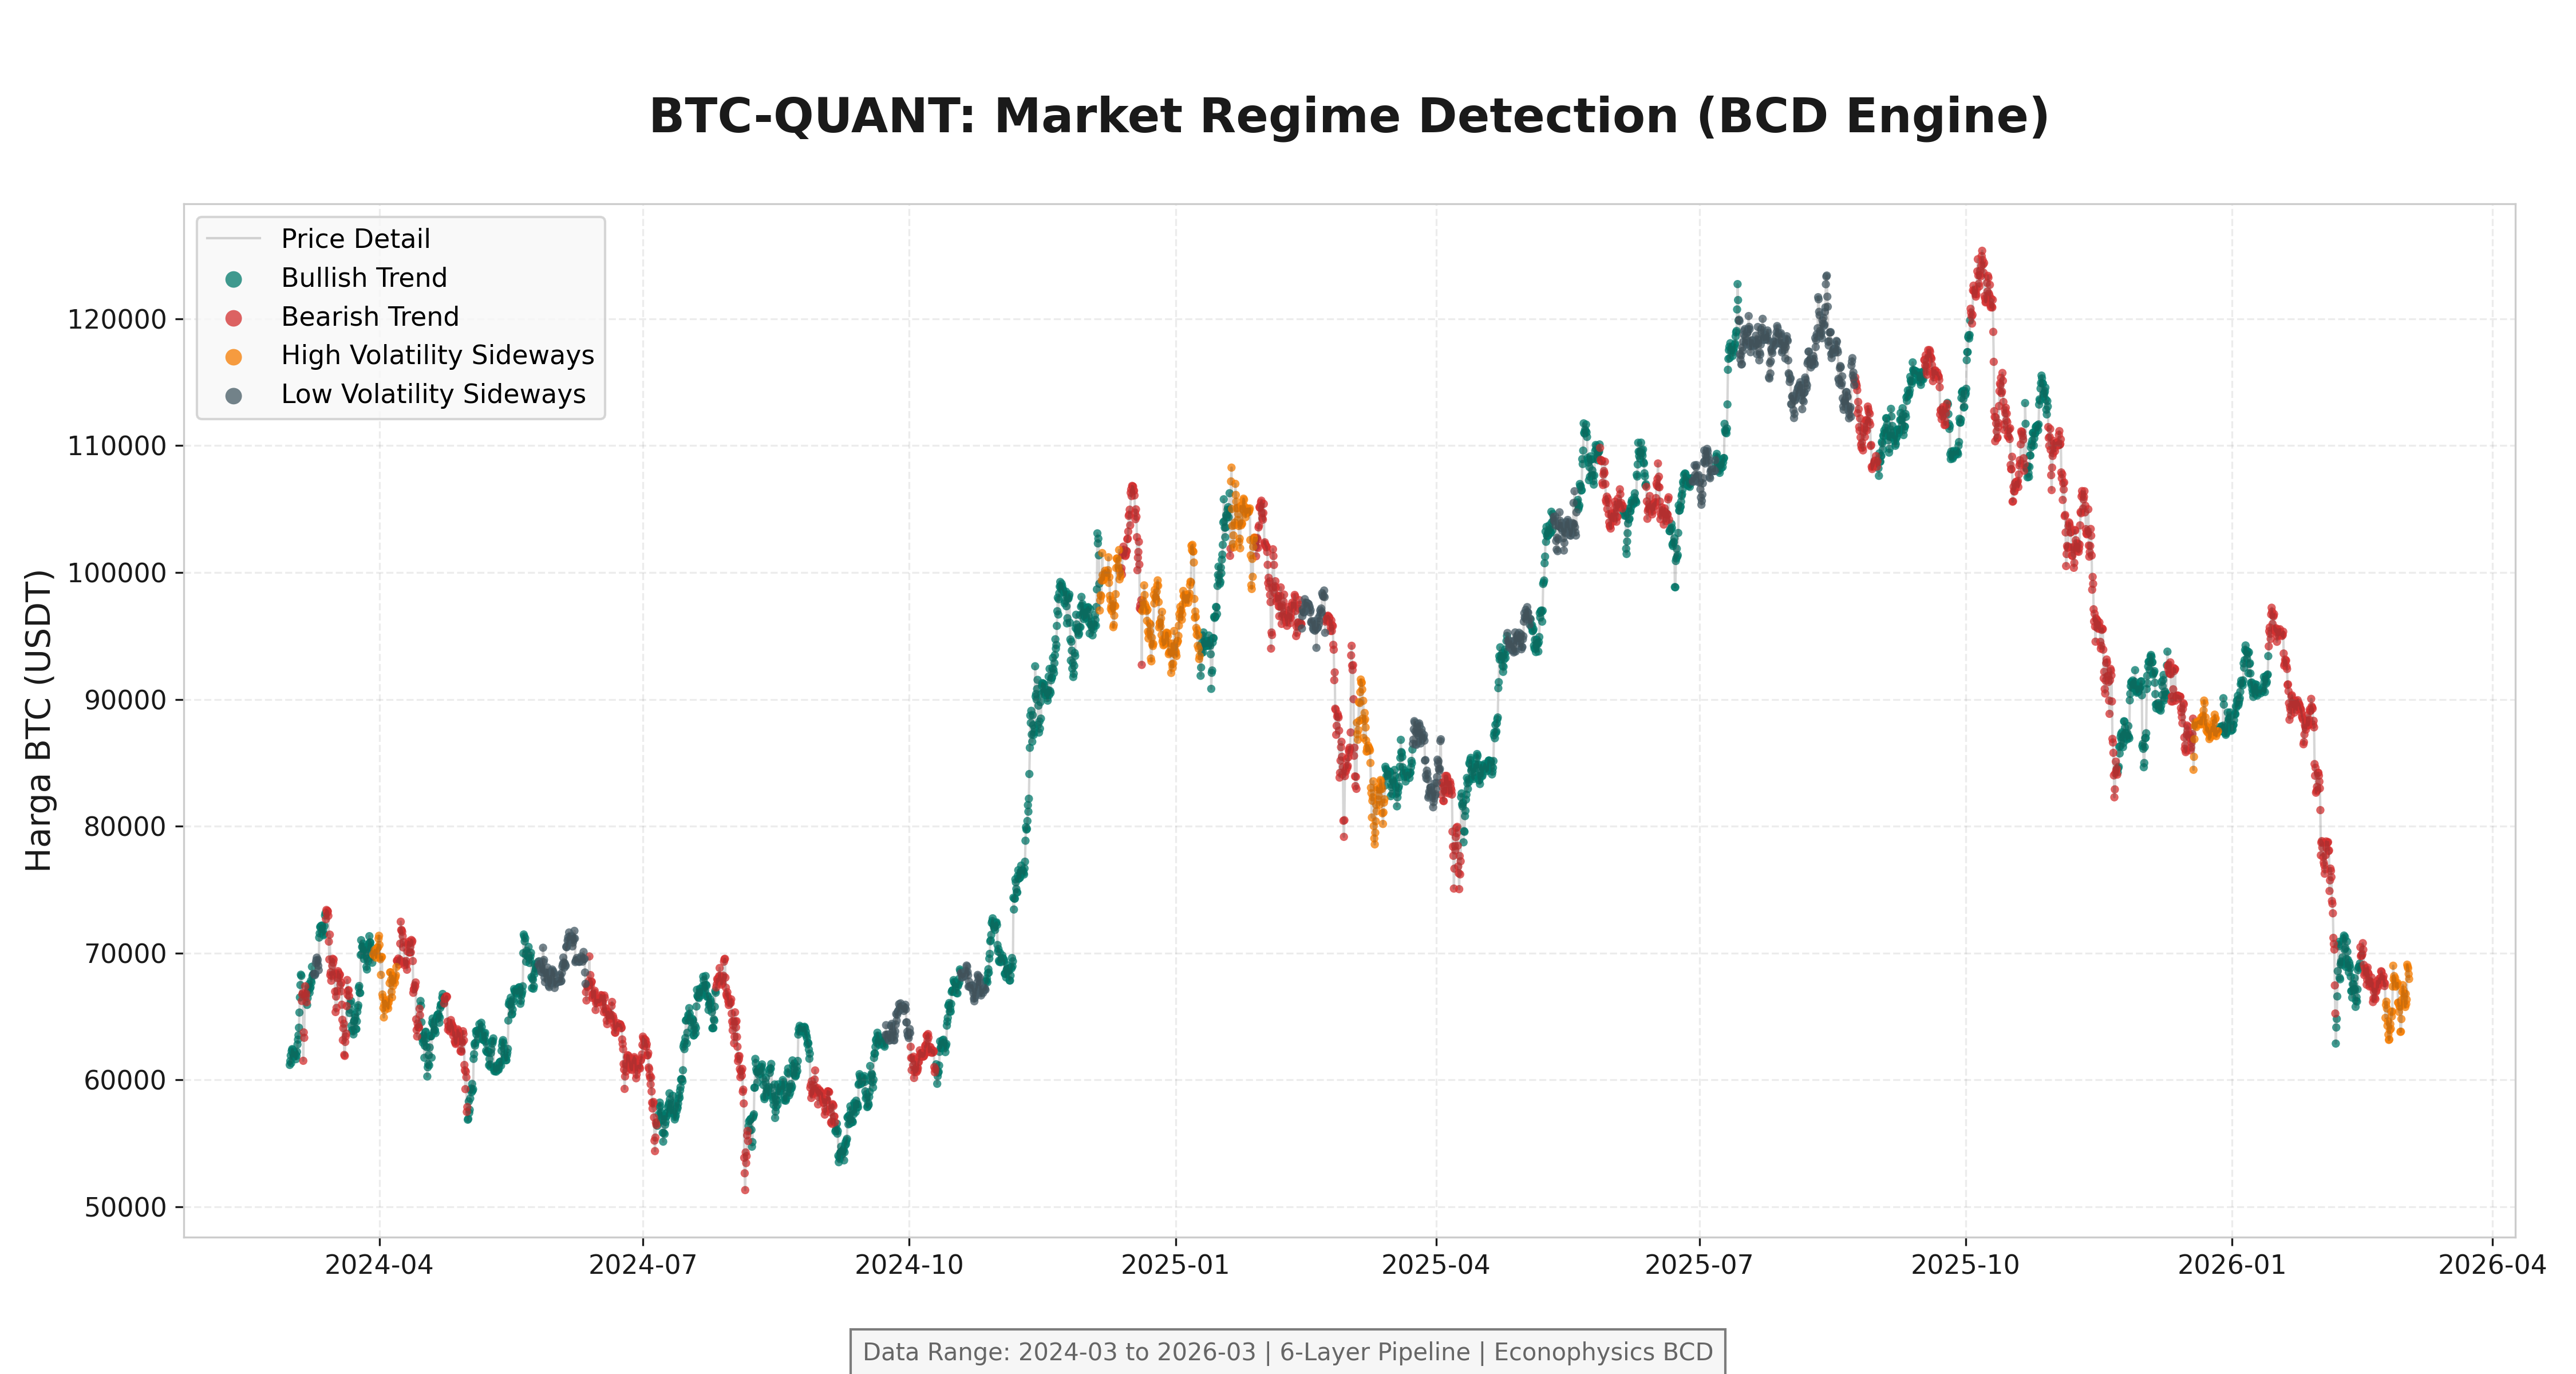
\includegraphics[width=0.9\textwidth]{figures/regime_plot.png}
    \caption{Visualisasi Plot Rezim Pasar Menggunakan Bayesian Changepoint Detection (BCD) pada Data BTC/USDT.}
    \label{fig:regime_plot}
\end{figure}

\begin{figure}[h!]
    \centering
    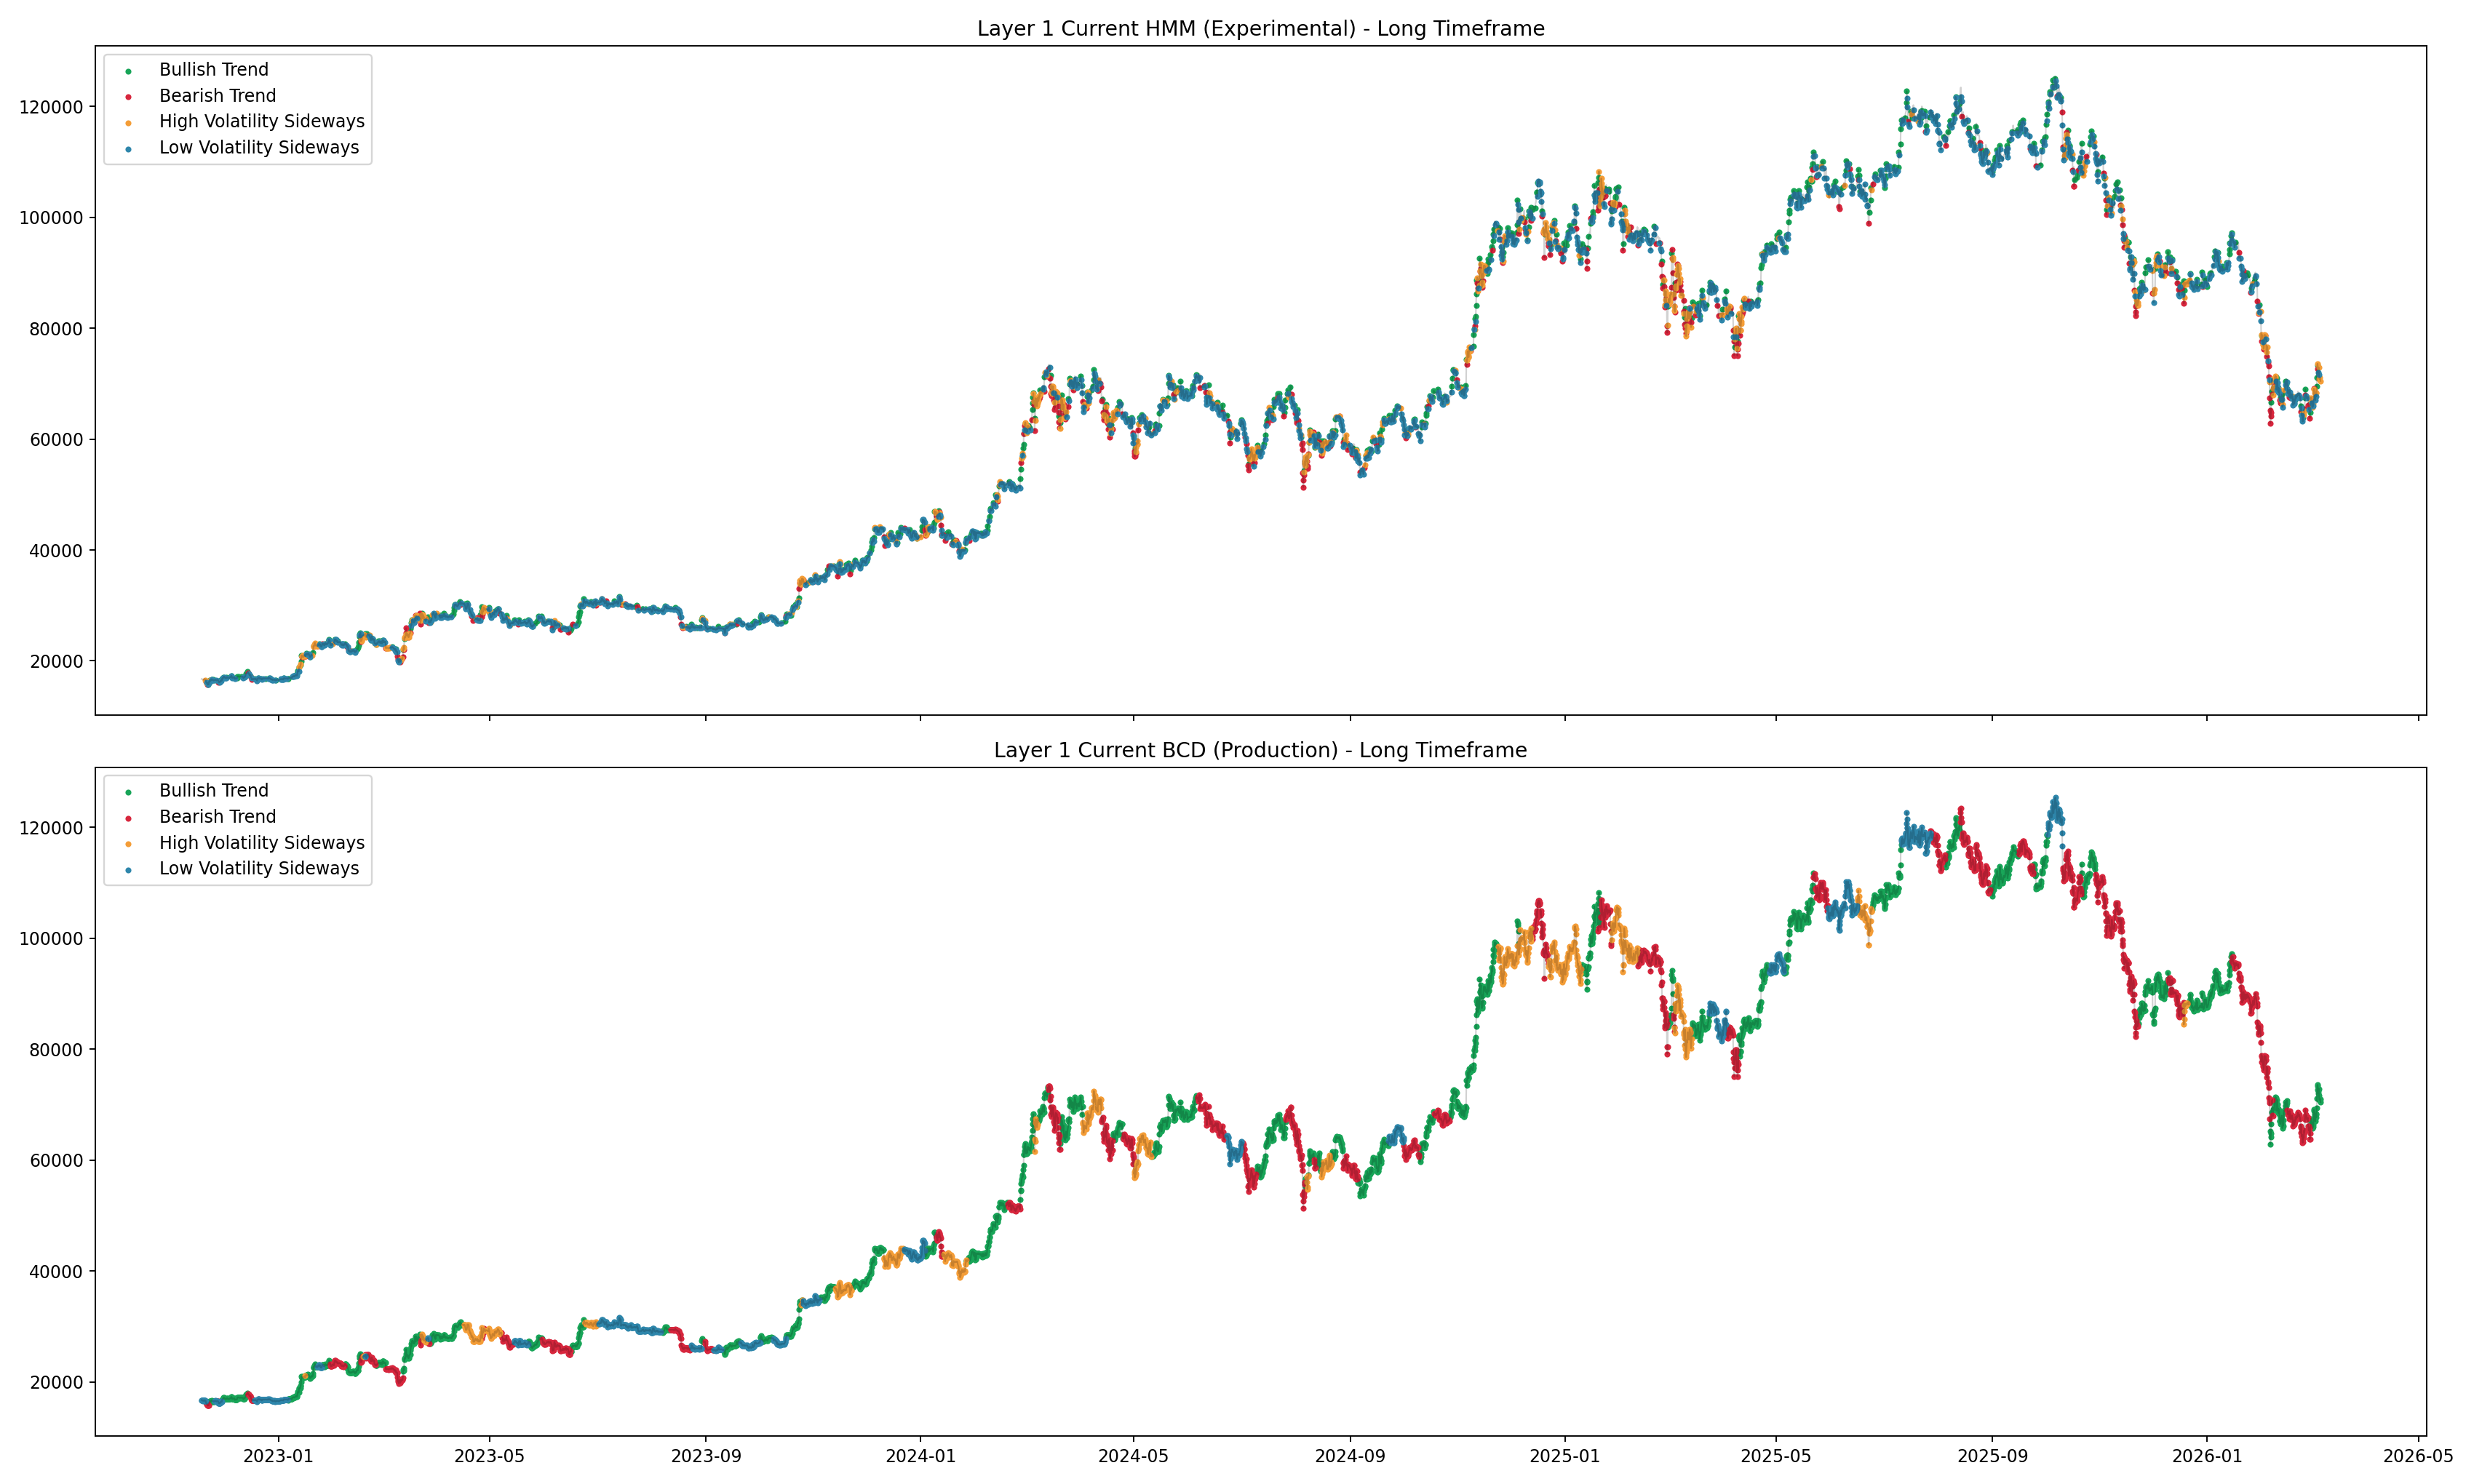
\includegraphics[width=0.9\textwidth]{figures/long_compare_viz.png}
    \caption{Perbandingan Kurva Ekuitas dan Drawdown Strategi BTC-QUANT v3 vs v4.4.}
    \label{fig:equity_comparison}
\end{figure}

Pengujian selama 793 hari membuktikan keunggulan arsitektur v4.4 dalam menjaga profil risiko yang sehat sambil tetap menghasilkan keuntungan yang konsisten.

\begin{table}[h!]
\centering
\caption{Metrik Performa Final BTC-QUANT v4.4}
\label{table:metrics}
\begin{tabular}{@{}ll@{}}
\toprule
\textbf{Metrik}          & \textbf{Nilai (v4.4)} \\ \midrule
Win Rate (WR)            & 58.07\%               \\
Net PnL (\%)             & +231.64\%             \\
Max Drawdown (MDD)       & 12.53\%               \\
Profit Factor (PF)       & 1.230                 \\
Sharpe Ratio             & 2.248                 \\
Daily Return             & 0.292\%               \\
Average Hold Time        & 11.6 jam (2.91c)      \\ \bottomrule
\end{tabular}
\end{table}

\subsection{Ketahanan Lintas Rezim Pasar}
Salah satu kekuatan utama dari pendekatan ekonofisika BCD adalah kemampuannya beradaptasi di berbagai kondisi pasar. Berikut adalah rincian performa berdasarkan deteksi rezim Layer 1 dari pengujian longitudinal 7 tahun (2019--2026, 3.866 \textit{trade}):

\begin{itemize}
    \item \textbf{Bull Market:} \textit{Win Rate} 59.9\% (2.305 \textit{trade}, kontribusi PnL +\$85.920). Memberikan kontribusi profit terbesar selama fase tren naik yang kuat.
    \item \textbf{Bear Market:} \textit{Win Rate} 56.2\% (1.561 \textit{trade}, kontribusi PnL +\$32.402). Tetap mencetak profit bersih di pasar yang menurun, membuktikan efektivitas filter arah (\textit{bias persistence}) dari Layer 1 BCD.
\end{itemize}

Konsistensi \textit{Win Rate} di atas 56\% pada kedua regime --- bahkan tanpa regime \textit{Sideways} yang terdeteksi dalam dataset 7 tahun --- mengonfirmasi bahwa \textit{Directional Spectrum} (Bab 3) secara efektif menyeleksi peluang dengan probabilitas tinggi di berbagai kondisi pasar.

% =========================================================
\subsection{Komparasi v4.4 vs Heston Adaptive v4.5: Walk-Forward 62 Hari}
\label{subsec:comparison_62d}

Sebagai lanjutan dari validasi Golden v4.4, dilakukan pengujian komparatif antara dua model secara paralel untuk mengukur dampak dari penambahan modul volatilitas adaptif Heston. Eksperimen ini dijalankan pada jendela pendek (62 hari) untuk mengisolasi performa tanpa efek compounding jangka panjang.

\textbf{Parameter Eksperimen:}
\begin{itemize}
    \item \textbf{Periode:} 1 Januari 2026 -- 4 Maret 2026 (62 hari)
    \item \textbf{Modal Awal:} \$10,000 masing-masing model
    \item \textbf{Model A (Golden v4.4):} SL tetap 1.333\%, TP tetap 0.71\%, leverage 15×, margin \$1,000/trade
    \item \textbf{Model B (Heston v4.5):} SL/TP adaptif berbasis ATR × multiplier, \textit{dynamic sizing} 2\% ekuitas/trade, leverage maks 5×
\end{itemize}

\begin{table}[h!]
\centering
\caption{Perbandingan Performa: Golden v4.4 vs Heston Adaptive v4.5 (62 Hari)}
\label{table:comparison_62d}
\begin{tabular}{@{}llll@{}}
\toprule
\textbf{Metrik}        & \textbf{Golden v4.4} & \textbf{Heston v4.5} & \textbf{Pemenang} \\ \midrule
Net PnL (\%)           & +30.04\%             & \textbf{+76.10\%}    & Heston \\
Final Equity (USD)     & \$13,004             & \textbf{\$17,610}    & Heston \\
Daily Return           & 0.485\%/hari         & \textbf{1.227\%/hari}& Heston \\
Win Rate               & \textbf{57.36\%}     & 49.35\%              & Golden \\
Profit Factor          & 1.278                & \textbf{1.587}       & Heston \\
Max Drawdown           & 20.75\%              & \textbf{17.10\%}     & Heston \\
Sharpe Ratio           & 2.299                & \textbf{3.409}       & Heston \\
R:R Ratio              & 0.950                & \textbf{1.629}       & Heston \\
Avg Winner (USD)       & \$186.67             & \textbf{\$541.38}    & Heston \\
Jumlah Trade           & \textbf{129}         & 77                   & Golden \\
\bottomrule
\end{tabular}
\end{table}

\textbf{Verdict: Heston menang 7 dari 10 metrik.} Model adaptif menghasilkan return \textbf{2.53× lebih tinggi} dengan drawdown yang lebih kecil. Kunci keunggulan Heston terletak pada tiga mekanisme struktural: (1) R:R yang lebih baik (1.63 vs 0.95) memberikan buffer keamanan lebih besar terhadap penurunan win rate; (2) \textit{dynamic position sizing} yang membatasi kerugian per trade ke 2\% ekuitas mencegah spiral drawdown; dan (3) SL/TP adaptif berbasis volatilitas aktual menghasilkan target yang lebih realistis per kondisi pasar.

Distribusi exit mengungkap satu peringatan penting: 36.4\% trade Heston keluar via \textit{TIME\_EXIT} (vs 7.0\% Golden), menandakan bahwa TP Heston terlalu ambisius untuk kondisi \textit{Low Vol} yang mendominasi periode Jan--Mar 2026.

% =========================================================
\subsection{Validasi Longitudinal 7 Tahun: Golden v4.4 vs Heston v4.5 (2019--2026)}
\label{subsec:longitudinal_7y}

Untuk mengevaluasi ketahanan kedua model terhadap berbagai siklus pasar Bitcoin, dilakukan pengujian longitudinal penuh mencakup 7 tahun data historis mulai dari fase \textit{bear market} awal 2019, lonjakan \textit{bull market} 2020--2021, siklus koreksi 2022, hingga pemulihan 2023--2026.

\textbf{Parameter Eksperimen:}
\begin{itemize}
    \item \textbf{Periode:} 18 November 2019 -- 4 Maret 2026 (2,619 hari, 13,783 candle 4H)
    \item \textbf{Modal Awal:} \$10,000 masing-masing model
    \item \textbf{Total Sinyal Dievaluasi:} Golden 11,132 (3,866 dieksekusi, 7,266 dilewati); Heston 8,951 (2,100 dieksekusi, 6,851 dilewati)
\end{itemize}

\begin{table}[h!]
\centering
\caption{Perbandingan Performa Longitudinal: Golden v4.4 vs Heston v4.5 (2019--2026)}
\label{table:longitudinal_7y}
\begin{tabular}{@{}llll@{}}
\toprule
\textbf{Metrik}          & \textbf{Golden v4.4} & \textbf{Heston v4.5}   & \textbf{Pemenang} \\ \midrule
Final Equity (USD)       & \$128,321            & \textbf{\$16,928,244}  & Heston \\
Net PnL (\%)             & +1,183\%             & \textbf{+169,182\%}    & Heston \\
Daily Return             & 0.452\%/hari         & \textbf{64.6\%/hari}   & Heston \\
R:R Ratio                & 0.976                & \textbf{1.488}         & Heston \\
Win Rate                 & \textbf{58.43\%}     & 46.67\%                & Golden \\
Profit Factor            & \textbf{1.372}       & 1.302                  & Golden \\
Max Drawdown             & \textbf{12.40\%}     & 71.94\%                & Golden \\
Sharpe Ratio             & \textbf{3.087}       & 1.007                  & Golden \\
Avg Winner (USD)         & \$193                & \textbf{\$74,481}      & Heston \\
Avg Loser (USD)          & \textbf{\$198}       & \$50,066               & Golden \\
Jumlah Trade             & 3,866                & 2,100                  & -- \\
Avg Hold Time            & 2.69 candle          & 4.30 candle            & -- \\
\bottomrule
\end{tabular}
\end{table}

\textbf{Verdict: Golden menang 6 dari 10 metrik.} Hasil ini tampak paradoks --- Heston menghasilkan ekuitas akhir \textbf{131× lebih besar} (\$16.9 juta vs \$128 ribu), namun kalah dalam metrik kualitas. Penjelasannya adalah efek \textit{compounding agresif} selama 7 tahun: setiap kemenangan Heston meningkatkan basis modal untuk trade berikutnya, menghasilkan pertumbuhan eksponensial.

Namun, keunggulan nominal ini datang dengan biaya yang signifikan:
\begin{itemize}
    \item \textbf{Max Drawdown 71.94\%} -- Pada titik terburuk, ekuitas Heston bisa menyusut hingga 72\% dari puncaknya. Sebuah akun \$16.9 juta bisa turun menjadi \$4.7 juta. Secara psikologis dan operasional, kondisi ini hampir mustahil dipertahankan tanpa intervensi.
    \item \textbf{Sharpe Ratio 1.007} -- Mendekati ambang batas minimum yang dapat diterima ($>$1.0). Return tinggi namun volatilitas yang ekstrem mengikis nilai risk-adjusted return.
    \item \textbf{TIME\_EXIT Rate 39.5\%} -- Hampir 4 dari 10 trade keluar via timeout (vs 5.4\% Golden). TP Heston yang adaptif terlalu ambisius untuk kondisi pasar rata-rata selama 7 tahun data.
    \item \textbf{High Vol Regime: Tidak Teruji} -- Seluruh 2,100 trade Heston dikategorikan sebagai regime \textit{Normal} atau \textit{Low Vol}. Multiplier SL/TP untuk kondisi \textit{High Vol} (×2.0/×1.5) sama sekali belum divalidasi secara empiris.
\end{itemize}

\begin{table}[h!]
\centering
\caption{Distribusi Exit: Golden v4.4 vs Heston v4.5 (2019--2026)}
\label{table:exit_dist_7y}
\begin{tabular}{@{}lllll@{}}
\toprule
\textbf{Exit Type} & \textbf{Golden (n)} & \textbf{Golden (\%)} & \textbf{Heston (n)} & \textbf{Heston (\%)} \\ \midrule
Stop Loss (SL)     & 1,446 & 37.4\% & 693  & 33.0\% \\
Trailing TP        & 1,261 & 32.6\% & 300  & 14.3\% \\
Full TP            & 952   & 24.6\% & 278  & 13.2\% \\
\textbf{TIME\_EXIT}& \textbf{207}   & \textbf{5.4\%}  & \textbf{829}  & \textbf{39.5\%} \\
\bottomrule
\end{tabular}
\end{table}

\begin{table}[h!]
\centering
\caption{Performa per Regime Pasar: Golden v4.4 vs Heston v4.5 (2019--2026)}
\label{table:regime_7y}
\begin{tabular}{@{}lllll@{}}
\toprule
\textbf{Model} & \textbf{Regime} & \textbf{Trades} & \textbf{Win Rate} & \textbf{Total PnL (USD)} \\ \midrule
Golden v4.4    & Bull            & 2,305           & 59.9\%            & +\$85,920 \\
Golden v4.4    & Bear            & 1,561           & 56.2\%            & +\$32,402 \\
Heston v4.5    & Bull            & 1,263           & 48.2\%            & +\$8,547,079 \\
Heston v4.5    & Bear            & 837             & 44.3\%            & +\$8,371,165 \\
\bottomrule
\end{tabular}
\end{table}

\subsubsection{Interpretasi Komparatif Lintas Horison Waktu}

Perbandingan dua horison waktu --- 62 hari vs 7 tahun --- menghasilkan kesimpulan yang saling melengkapi:

\begin{enumerate}
    \item \textbf{Jangka Pendek (62 hari):} Heston lebih baik di hampir semua dimensi kualitas (Sharpe, drawdown, profit factor) \textbf{dan} lebih profitable. Ini adalah kondisi ideal untuk deployment.
    \item \textbf{Jangka Panjang (7 tahun):} Keunggulan Heston dalam return nominal sangat besar (+169,182\% vs +1,183\%), tetapi kualitas metrik risk-adjusted (Sharpe, drawdown) memburuk secara drastis akibat compounding eksponensial yang memperbesar risiko seiring waktu.
    \item \textbf{Konsistensi Golden:} Golden mempertahankan Sharpe $>$3.0 dan drawdown $<$12.5\% bahkan setelah 7 tahun --- bukti stabilitas arsitektur yang tidak terdegradasi lintas siklus pasar.
\end{enumerate}

\textbf{Kesimpulan praktis:} Untuk akun produksi dengan batasan risiko institusional (drawdown $<$20\%), Golden v4.4 adalah pilihan yang lebih aman. Untuk akun eksplorasi dengan toleransi risiko tinggi dan horison panjang, Heston v4.5 menawarkan potensi return eksponensial yang belum tertandingi --- dengan catatan bahwa regime \textit{High Vol} masih merupakan \textit{blind spot} yang harus divalidasi sebelum deployment penuh.

\section{Kesimpulan dan Roadmap Selanjutnya}
\label{sec:conclusion}

Dokumentasi teknis ini merangkum seluruh perjalanan inovasi dan transformasi arsitektur BTC-QUANT. Kami telah membuktikan bahwa keberhasilan dalam perdagangan algoritmik di pasar Bitcoin tidak bergantung pada indikator teknikal yang kompleks, melainkan pada pemahaman mendalam terhadap struktur fisik pasar dan manajemen risiko yang stabil.

\subsection{Intisari Pembelajaran}
Berikut adalah poin-poin kesimpulan strategis dari pengembangan ini:
\begin{enumerate}
    \item \textbf{Ekonofisika > Machine Learning Klasik:} Pengenalan BCD dan distribusi Student-T terbukti lebih efektif dalam menangani fenomena \textit{non-stationary} pasar kripto dibandingkan model Markovian konvensional.
    \item \textbf{Stability is the New High Return:} Dengan menekan \textit{Max Drawdown} ke angka 12.53\%, sistem ini menawarkan profil risiko-pengembalian (\textit{Sharpe Ratio} 2.24) yang unggul di atas model mana pun yang lebih agresif.
    \item \textbf{Simplisitas di Atas Kompleksitas:} Versi 4.4 Golden Model yang murni tanpa mekanisme \textit{lock-in} tambahan terbukti paling stabil, memberikan pelajaran bahwa strategi terbaik sering kali adalah strategi yang menyisakan ruang bagi dinamika alami pasar.
\end{enumerate}

\subsection{Roadmap Pengembangan}

Meskipun \textit{Golden Model} v4.4 telah mencapai standar produksi, pengembangan sistem terus berlanjut. Fase R\&D saat ini telah menghasilkan \textbf{v4.5 Heston Adaptive} --- varian eksperimental yang mengintegrasikan model volatilitas stokastik Heston untuk kalibrasi SL/TP adaptif dan \textit{dynamic position sizing} berbasis Kriteria Kelly. Hasil pengujian awal menunjukkan potensi yang signifikan, namun terdapat satu prasyarat kritis yang harus dipenuhi sebelum \textit{deployment} penuh.

Prioritas pengembangan ke depan adalah sebagai berikut:
\begin{itemize}
    \item \textbf{Validasi \textit{High Volatility Regime} (Prioritas Utama):} Seluruh 2.100 \textit{trade} v4.5 dalam pengujian 7 tahun dikategorikan sebagai regime \textit{Normal} atau \textit{Low Vol}. \textit{Multiplier} SL/TP untuk kondisi \textit{High Volatility} ($\times$2.0/$\times$1.5) belum pernah diuji secara empiris dan merupakan \textit{blind spot} yang harus diselesaikan sebelum v4.5 layak untuk produksi.
    \item \textbf{Kalibrasi Parameter Heston per Siklus Pasar:} Parameter $\gamma$, $\eta$, dan $\kappa$ pada model Heston saat ini dikalibrasi secara global. Kalibrasi adaptif per regime (bull/bear/sideways) berpotensi meningkatkan akurasi estimasi volatilitas secara signifikan.
    \item \textbf{Sentiment Aggregation (Layer 5):} Mengintegrasikan data sentimen pasar (\textit{Fear \& Greed Index}, \textit{funding rate}, \textit{open interest}) sebagai lapisan konfirmasi tambahan untuk memitigasi risiko peristiwa \textit{Black Swan} yang bersifat fundamental.
    \item \textbf{Eksekusi \textit{Real-Time}:} Migrasi dari simulasi \textit{backtest} ke modul eksekusi \textit{live} dengan koneksi API Binance WebSocket yang teroptimasi untuk latensi rendah.
\end{itemize}

Dengan landasan ekonofisika yang telah tervalidasi secara empiris dan arsitektur yang terbukti stabil lintas siklus pasar, BTC-QUANT v4.4 siap menjadi basis sistem perdagangan algoritmik institusional, sementara v4.5 terus dikembangkan sebagai generasi berikutnya dengan potensi pertumbuhan eksponensial yang terkontrol.


% --- References ---
\bibliographystyle{plain}
\bibliography{references}

\end{document}
